\documentclass[10pt,journal,compsoc]{IEEEtran}
%\usepackage{algorithm}
%\usepackage[noend]{algorithmic}
\usepackage{latexsym}
\usepackage{amsfonts}
\usepackage{amsmath}
\usepackage{amssymb}
\usepackage{color}
\usepackage{epsfig}
\usepackage{xspace}
\usepackage{graphicx}
%\usepackage{times}
\usepackage{subfigure}
\usepackage{cite}
\usepackage[english]{babel}
\usepackage{balance}  % for  \balance command ON LAST PAGE  (only there!)

%%%%%%%%%%%%%%%%%%%%%%%%%%%%%%%%%%%%%
%% DO NOT DELETE!!
%%%%%%%%%%%%%%%%%%%%%%%%%%%%%%%%%%%%%
%\usepackage{tikz}
%\usetikzlibrary{trees}

\usepackage{epsfig}
\usepackage{multirow}
\usepackage{url}

\newcommand{\imp}{\vdash_{\cal I}}


%%%%%%%%%%%%%%%%%%%%%%%%%%%%%%%%%%%%%%%%%%
% Enumerate and Itemize modifications
\usepackage{enumitem}
\setlist{topsep=0pt,noitemsep} \setitemize[1]{label=$\circ$}
%%%%%%%%%%%%%%%%%%%%%%%%%%%%%%%%%%%%%%%%%%%

\sloppy
\newcommand{\rtable}[1]{\ensuremath{\mathsf{#1}}}
\newcommand{\ratt}[1]{\ensuremath{\mathit{#1}}}
\newcommand{\at}[1]{\protect\ensuremath{\mathsf{#1}}\xspace}
\newcommand{\myhrule}{\rule[.5pt]{\hsize}{.5pt}}
\newcommand{\oneurl}[1]{\texttt{#1}}
\newcommand{\eat}[1]{}
\newcommand{\stab}{\rule{0pt}{8pt}\\[-1.6ex]}
\newcommand{\sttab}{\rule{0pt}{8pt}\\[-2ex]}
\newcommand{\sstab}{\rule{0pt}{8pt}\\[-2.4ex]}
\newcommand{\tabstrut}{\rule{0pt}{4pt}\vspace{-0.07in}}
\newcommand{\vs}{\vspace{1ex}}
\newcommand{\exa}[2]{{\tt\begin{tabbing}\hspace{#1}\=\+\kill #2\end{tabbing}}}
\newcommand{\ra}{\rightarrow}
\newcommand{\la}{\leftarrow}
\newcommand{\bi}{\begin{itemize}}
\newcommand{\ei}{\end{itemize}}
\newenvironment{tbi}{\begin{itemize}
        \setlength{\topsep}{1.5ex}\setlength{\itemsep}{0ex}\vspace{-0.5ex}}
        {\end{itemize}\vspace{-0.5ex}}
\newenvironment{tbe}{\begin{enumerate}
        \setlength{\topsep}{0ex}\setlength{\itemsep}{-0.7ex}\vspace{-1ex}}
        {\end{itemize}\vspace{-1ex}}

\newcommand{\mat}[2]{{\begin{tabbing}\hspace{#1}\=\+\kill #2\end{tabbing}}}
\newcommand{\m}{\hspace{0.05in}}
\newcommand{\ls}{\hspace{0.1in}}
\newcommand{\be}{\begin{enumerate}}
\newcommand{\ee}{\end{enumerate}}
\newcommand{\beqn}{\begin{eqnarray*}}
\newcommand{\eeqn}{\end{eqnarray*}}
\newcommand{\card}[1]{\mid\! #1\!\mid}
\newcommand{\fth}{\hfill $\Box$}
\newcommand{\AND}{\displaystyle{\bigwedge_{i=1}^{n}}}
\newcommand{\U}[1]{\displaystyle{\bigcup_{#1}}}
\newcommand{\Sm}[1]{\displaystyle{\sum_{#1}}}
\newcommand{\stitle}[1]{\vspace{1ex}\noindent{\bf #1}}
\newcommand{\etitle}[1]{\vspace{0.8ex}\noindent{\em \underline{#1}}}
\renewcommand{\t}{\tau}
\newcommand{\Inh}[1]{\$#1}
\renewcommand{\r}[1]{{\it rule}(#1)}
\newcommand{\pa}{\parallel}
\newcommand{\LHS}{\kw{{\small LHS}}}
\newcommand{\RHS}{\kw{RHS}}
\newcommand{\len}{\kw{len}}
\newcommand{\kop}{\kw{op}}
\newcommand{\ie}{\emph{i.e.,}\xspace}
\newcommand{\eg}{\emph{e.g.,}\xspace}
\newcommand{\wrt}{\emph{w.r.t.}\xspace}
\newcommand{\aka}{\emph{a.k.a.}\xspace}
\newcommand{\kwlog}{\emph{w.l.o.g.}\xspace}
%%%%%%%%%%%%%%%%%%%%%%%%%%%%%%%%%%%%%%%%%%%%%%%%%%%%%%%%%%%%%%%%
%                  Relation Algebra operators
%%%%%%%%%%%%%%%%%%%%%%%%%%%%%%%%%%%%%%%%%%%%%%%%%%%%%%%%%%%%%%%%

\newcommand{\RS}{{\small S}\xspace}
\newcommand{\RP}{{\small P}\xspace}
\newcommand{\RJ}{{\sc j}\xspace}
\newcommand{\RC}{{\small C}\xspace}
\newcommand{\RSJ}{{\small SJ}\xspace}
\newcommand{\RSC}{{\small SC}\xspace}
\newcommand{\RSP}{{\small SP}\xspace}
\newcommand{\RPJ}{{\small PJ}\xspace}
\newcommand{\RPC}{{\small PC}\xspace}
\newcommand{\RSPJ}{{\sc spj}\xspace}
\newcommand{\RSPC}{{\small SPC}\xspace}
\newcommand{\RSPJU}{{\sc spju}\xspace}
\newcommand{\RSPCU}{{\small SPCU}\xspace}
\newcommand{\RSPJUN}{{\small SPJU$^N$}\xspace}
\newcommand{\RSPCUN}{{\small SPCU$^N$}\xspace}
%%%%%%%%%%%%%%%%%%%%%%%%%%%%%%%%%%%%%%%%%%%%%%%%%%%%%%%%%%%%%%%%%%%%%%%%%%%%%%
% ALGORITHMS
%%%%%%%%%%%%%%%%%%%%%%%%%%%%%%%%%%%%%%%%%%%%%%%%%%%%%%%%%%%%%%%%%%%%%%%%%%%%%%%
\newcommand{\SELECT}{\mbox{{\bf select}}\ }
\newcommand{\FROM}{\mbox{{\bf from}\ }}
\newcommand{\WHERE}{\mbox{\bf where}\ }
\newcommand{\SUM}{\mbox{{\bf sum}}\ }
\newcommand{\GROUPBY}{\mbox{{\bf group by}}\ }
\newcommand{\HAVING}{\mbox{{\bf having}}\ }
\newcommand{\CASE}{\mbox{{\bf case}}\ }
\newcommand{\END}{\mbox{{\bf end}}\ }
\newcommand{\WHEN}{\mbox{{\bf when}}\ }
\newcommand{\EXISTS}{\mbox{{\bf exists}}\ }
\newcommand{\COUNT}{\mbox{\kw{count}}}
\newcommand{\INSERTINTO}{\mbox{{\bf insert into}}\ }
\newcommand{\UPDATE}{\mbox{{\bf update}}\ }
\newcommand{\SET}{\mbox{{\bf set}}\ }
\newcommand{\IN}{\mbox{{\bf in}}\ }
\newcommand{\If}{\mbox{\bf if}\ }
\newcommand{\Let}{\mbox{\bf let}\ }
\newcommand{\Call}{\mbox{\bf call}\ }
\newcommand{\Then}{\mbox{\bf then}\ }
\newcommand{\To}{\mbox{\bf to}\ }
\newcommand{\Else}{\mbox{\bf else}\ }
\newcommand{\ElseIf}{\mbox{\bf elseif}\ }
\newcommand{\While}{\mbox{\bf while}\ }
\newcommand{\Begin}{\mbox{\bf begin}\ }
\newcommand{\End}{\mbox{\bf end}\ }
\newcommand{\Do}{\mbox{\bf do}\ }
\newcommand{\Downto}{\mbox{\bf downto}\ }
\newcommand{\Repeat}{\mbox{\bf repeat}\ }
\newcommand{\Until}{\mbox{\bf until}\ }
\newcommand{\For}{\mbox{\bf for}\ }
\newcommand{\Each}{\mbox{\bf each}\ }

\newcommand{\ForEach}{\mbox{\bf for each}\ }
\newcommand{\Or}{\mbox{\bf or}\ }
\renewcommand{\And}{\mbox{\bf and}\ }
\newcommand{\Not}{\mbox{\bf not}\ }
\newcommand{\Break}{\mbox{\bf break}\ }
\newcommand{\Continue}{\mbox{\bf continue}\xspace}
\newcommand{\Return}{\mbox{\bf return}\ }
\newcommand{\Case}{\mbox{\bf case}\ }
\newcommand{\Of}{\mbox{\bf of}\ }
\newcommand{\EndCase}{\mbox{\bf end-case}\ }
\newcommand{\NIL}{\mbox{\em nil}}
\newcommand{\False}{\mbox{\em false}}
\newcommand{\True}{\mbox{\em true}}
\newcommand{\algAND}{{\sc and}\xspace}
\newcommand{\OR}{{\sc or}\xspace}
\newcommand{\NOT}{{\sc not}\xspace}
\newcommand{\kw}[1]{{\ensuremath {\mathsf{#1}}}\xspace}

\newcounter{ccc}
\newcommand{\bcc}{\setcounter{ccc}{1}\theccc.}
\newcommand{\icc}{\addtocounter{ccc}{1}\theccc.}
\newcommand{\checking}{{\mbox{\small\sf Checking}\xspace}}
\newcommand{\preProcessing}{{\mbox{\small\sf preProcessing}\xspace}}
\newcommand{\CFDconsistency}{{\mbox{\s%\documentclass{vldb}
\documentclass{sig}
\usepackage{algorithm}
\usepackage[noend]{algorithmic}
\usepackage{latexsym}
\usepackage{amsfonts}
\usepackage{amsmath}
\usepackage{amssymb}
\usepackage{color}
\usepackage{epsfig}
\usepackage{xspace}
\usepackage{graphicx}
\usepackage{times}
\usepackage{subfigure}mall\sf CFD\_Checking}\xspace}}
\newcommand{\MCS} {\kw{MCS}}
\newcommand{\templateDB}{{\mbox{\small\sf templateDB}\xspace}}
\newcommand{\ChaseChecking}{{\mbox{\small\sf RandomChecking}\xspace}}
\newcommand{\chase}{{\mbox{\small\sf Chase}\xspace}}
\newcommand{\SAT}{{\mbox{\small\sf SAT}\xspace}}
\newcommand{\kSAT}{{\mbox{\small 3SAT}\xspace}}
\newcommand{\PropCFDSPC}{\kw{Prop{\small CFD\_SPC}}}
\newcommand{\PropCFDSPCU}{\kw{Prop{\small CFD\_SPCU}}}
\newcommand{\UnionEQs}{\kw{UnionEQs}}
\newcommand{\UnionCFDs}{\kw{UnionCFDs}}
\newcommand{\EQ}{\kw{EQ}}
\newcommand{\eq}{\kw{eq}}
\newcommand{\key}{\kw{key}}
\newcommand{\rep}{\kw{rep}}
\newcommand{\PEQ}{\kw{EQ2CFD}}
\newcommand{\Drop}{\kw{Drop}}
%\newcommand{\Res}{\kw{Res}}
\newcommand{\CFD}{{\small CFD}\xspace}
\newcommand{\CFDs}{{\small CFD}{\small s}\xspace}
\newcommand{\CIND}{{\sc cind}\xspace}
\newcommand{\cind}{{\small \sf CIND}}
\newcommand{\cfd}{{\small \sf CFD}}
\newcommand{\CINDp}{{\sc cind}$^+$\xspace}
\newcommand{\CINDn}{{\sc cind}$^-$\xspace}
\newcommand{\CINDs}{{\sc cind}{\small s}\xspace}
\newcommand{\FD}{{\small FD}\xspace}
\newcommand{\FDs}{{\small FD}{\small s}\xspace}
\newcommand{\IND}{{\sc ind}\xspace}
\newcommand{\INDs}{{\sc ind}{\small s}\xspace}
\newcommand{\TGDs}{{\sc tgd}{\small s}\xspace}
\newcommand{\NP}{{\sc np}\xspace}
\newcommand{\DAGs}{{\sc dag}s\xspace}
\newcommand{\NC}{{\sc nc}\xspace}
\newcommand{\coNP}{co{\sc np}\xspace}
\newcommand{\PTIME}{{\sc ptime}\xspace}
\newcommand{\PSPACE}{{\sc pspace}\xspace}
\newcommand{\EXPTIME}{{\sc exptime}\xspace}
\newcommand{\NPSPACE}{{\sc npspace}\xspace}
\newcommand{\dom}{\protect\ensuremath{\mathsf{dom}}\xspace}
\newcommand{\atset}{\protect\ensuremath{\mathsf{attr}}\xspace}
\newcommand{\attr}[1]{\protect\ensuremath{\mathsf{#1}}\xspace}
\newcommand{\attrset}{\protect\ensuremath{\mathsf{attr}}\xspace}
\newcommand{\finatset}{\protect\ensuremath{\mathsf{finattr}}\xspace}
\newcommand{\pvar}{\protect\ensuremath{\mathsf{var\%}}\xspace}
\newcommand{\lLHS}{\protect\ensuremath{\mathsf{{\small LHS}}}\xspace}
\newcommand{\RA}{{\small RA}\xspace}
\newcommand{\RBR}{\kw{RBR}}
\newcommand{\SQL}{{\sc sql}\xspace}
\newcommand{\XSLT}{{\sc xslt}\xspace}
\newcommand{\DBMS}{{\sc dbms}\xspace}
\newcommand{\ATG}{{\sc atg}\xspace}
\newcommand{\ATGs}{{\sc atg}{\small s}\xspace}
\newcommand{\EBI}{{\sc ebi}\xspace}
\newcommand{\GO}{{\sc go}\xspace}
\newcommand{\VEC}[1]{{\sc vec}(#1)}
\newcommand{\DAG}{{\sc dag}\xspace}
\newcommand{\XQ}{{\sc xq}\xspace}
\newcommand{\XQwc}{{\sc xq}$^{\scriptscriptstyle[*]}$\xspace}
\newcommand{\XQdes}{{\sc xq}$^{\scriptscriptstyle[//]}$\xspace}
\newcommand{\XQfull}{{\sc xq}$^{\scriptscriptstyle[*,//]}$\xspace}
\newcommand{\vect}[1]{$\langle$ #1 $\rangle$}
\newcommand{\sem}[1]{[\![#1]\!]}
\newcommand{\NN}[2]{#1\sem{#2}}
\newcommand{\e}[2]{{\mathit (#1,#2)}}
\newcommand{\ep}[2]{{\mathit (#1,#2)+}}
\newcommand{\brname}{\ensuremath{{\mathsf{N}}}}
\newcommand{\budrel}[1]{\ensuremath{{\brname_{#1}}}}
\newcommand{\budgen}[2]{\ensuremath{Q^\brname_\e{#1}{#2}}}
\newcommand{\budcut}[2]{\ensuremath{Q_\e{#1}{#2}}}
\newcommand{\R}{{\cal R}}
\newcommand{\G}{{\cal G}}
\newcommand{\I}{{\cal I}}
\newcommand{\V}{{\cal V}}
\newcommand{\E}{{\cal E}}
\newcommand{\eop}{\hspace*{\fill}\mbox{$\Box$}}     % End of proof
\newcounter{example}
\renewcommand{\theexample}{\arabic{example}}
\newenvironment{example}{
        \vspace{1.5ex}
        \refstepcounter{example}
        {\noindent\bf Example \theexample:}}{
        \eop\vspace{1.5ex}}
\def\copyrightspace{}
\renewcommand{\ni}{\noindent}
\newcommand{\comlore}[1]{\begin{minipage}{3in}\fbox{\fbox{\parbox[t]{3in}{{\vspace{2mm}\noindent \bf COMM(LORE):~
{ #1}\hfill  END.}}}}\end{minipage}\\}
\newcommand{\comwenfei}[1]{\begin{minipage}{3in}\fbox{\fbox{\parbox[t]{3in}{{\vspace{2mm}\noindent \bf COMM(WENFEI):~
{ #1}\hfill  END.}}}}\end{minipage}\\}
\newcommand{\comshuai}[1]{\begin{minipage}{3in}\fbox{\fbox{\parbox[t]{3in}{{\vspace{2mm}\noindent \bf COMM(SHUAI):~
{ #1}\hfill  END.}}}}\end{minipage}\\}
\newcommand{\nthesection}{\arabic{section}}
\newcounter{theorem}
\renewcommand{\thetheorem}{\arabic{theorem}}
\newcounter{prop}
\renewcommand{\theprop}{\arabic{theorem}}
\newcounter{lemma}
\renewcommand{\thelemma}{\arabic{theorem}}
\newcounter{cor}
\renewcommand{\thecor}{\arabic{theorem}}
\newenvironment{theorem}{\begin{em}
        \refstepcounter{theorem}
        {\vspace{1.5ex} \noindent\bf  Theorem  \thetheorem:}}{
        \end{em}\eop\vspace{1.5ex}} %\hspace*{\fill}\vspace*{1ex}}
\newenvironment{prop}{\begin{em}
        \refstepcounter{theorem}
        {\vspace{1.5ex}\noindent \bf Proposition \theprop:}}{
        \end{em}\eop\vspace{1.5ex}}%\hspace*{\fill}\vspace*{1ex}}
\newenvironment{lemma}{\begin{em}
        \refstepcounter{theorem}
        {\vspace{1ex}\noindent\bf Lemma \thelemma:}}{
        \end{em}\eop\vspace{1ex}} %\hspace*{\fill}\vspace*{1ex}}
\newenvironment{cor}{\begin{em}
        \refstepcounter{theorem}
        {\vspace{1.5ex}\noindent\bf Corollary \thecor:}}{
        \end{em}\eop\vspace{1.5ex}} %\hspace*{\fill}\vspace*{1ex}}
\newcounter{definition}[section]
\renewcommand{\thedefinition}{\nthesection.\arabic{definition}}
\newenvironment{definition}{
        \vspace{1.5ex}
        \refstepcounter{definition}
        {\noindent\bf Definition {\bf \thedefinition}:}}{\eop\vspace{1.5ex}
}
\newcounter{alg}[section]
\renewcommand{\thealg}{\nthesection.\arabic{alg}}
\newenvironment{alg}[1]{
        \refstepcounter{alg}
        {\vspace{1ex}\noindent\bf Algorithm \thealg:\, #1}}{
        \vspace*{1ex}}
\newcounter{arule}
\renewcommand{\thearule}{\arabic{arule}}
\newenvironment{arule}{
        \vspace{0.6ex}
        \refstepcounter{arule}
        {\noindent \em Rule \thearule:}}{
        }
\newcounter{claim}
\renewcommand{\theclaim}{\arabic{claim}}
\newenvironment{claim}{
        \vspace{0.6ex}
        \refstepcounter{claim}
        {\noindent\em Claim \theclaim:}}{%--{ Wenfei Fan}\\
        }
\newenvironment{proof}{
        \vspace{1ex}
        {\noindent\bf Proof:}}{\eop\vspace{1ex}}
\newenvironment{proofS}{
        \vspace{1ex}
        {\noindent\bf Proof sketch:\ }}{\eop\vspace{1ex}}
\newenvironment{property}{
        \vspace{1ex}
        {\noindent\bf Property:}}{\eop\vspace{1ex}}

\newcommand{\SIM}{\ensuremath{\mathsf{mat}}}

\newcommand{\SIMe}{\ensuremath{\mathsf{mat_e}}}

\newcommand{\qual}{\kw{qual}}
\newcommand{\MaxCard}{\kw{qualCard}}
\newcommand{\MaxSim}{\kw{qualSim}}

\newcommand{\Rees}{R_{(e,e)}}
% \newcommand{\Reps}{R_{(e,p)}}
% \newcommand{\Rpps}{R_{(p,p)}}
% \newcommand{\ees}{\preceq_{(e,e)}}
% \newcommand{\eps}{\preceq_{(e,p)}}
% \newcommand{\nees}{\not\preceq_{e,e}}
% \newcommand{\neps}{\not\preceq_{e,p}}
% \newcommand{\pps}{\preceq_{(p,p)}}
% \newcommand{\bees}{\preceq^\mathsf{bw}_{(e,e)}}
% \newcommand{\nbees}{\not\preceq^\mathsf{bw}_{(e,e)}}
% \newcommand{\beps}{\preceq^\mathsf{bw}_{(e,p)}}
% \newcommand{\nbeps}{\not\preceq^\mathsf{bw}_{(e,p)}}

% \newcommand{\iees}{\precsim^{1-1}_{(e,e)}}
% \newcommand{\ieps}{\precsim^{1-1}_{(e,p)}}
% \newcommand{\sees}{\precsim_{(e,e)}}
% \newcommand{\seps}{\precsim^s_{(e,p)}}
% \newcommand{\nseps}{\not\precsim^s_{(e,p)}}
% \newcommand{\nieps}{\not\precsim^{1-1}_{(e,p)}}
% \newcommand{\oees}{\precsim^{\kw{opt}}_{(e,e)}}
% \newcommand{\oeps}{\precsim^{\kw{opt}}_{(e,p)}}
% \newcommand{\bsees}{\precsim^\mathsf{bw}_{(e,e)}}
% \newcommand{\bseps}{\precsim^\mathsf{bw}_{(e,p)}}
% \newcommand{\compPSim}{\kw{compPSim}}

%\newcommand{\URL} {\kw{URL}}
%\newcommand{\URLs} {\kw{URLs}}
\newcommand{\WIS} {\kw{WIS}}
\newcommand{\IS} {\kw{IS}}
\newcommand{\AFPR}{\kw{AFP}-\kw{reduction}}
\newcommand{\AFPRs}{\kw{AFP}-\kw{reductions}}

\newcommand{\OPT}{\kw{opt}}
\newcommand{\obj}{\kw{obj}}
\newcommand{\N} {{\cal N}}

\newcommand{\maxCSPS} {\kw{compMaxCard^s}}
\newcommand{\maxCSPI} {\kw{compMaxCard^{1-1}}}
\newcommand{\maxSSPS} {\kw{compMaxSim^s}}
\newcommand{\maxSSPI} {\kw{compMaxSim^{1-1}}}
\newcommand{\subIso} {\kw{cdkMCS}}
\newcommand{\combine} {\kw{combinedMaxSim}}


%\newcommand{\pSim}{\kw{compSimilarity}}
\newcommand{\gSim}{\kw{graphSimulation}}

\newcommand{\maxWIS} {\kw{compMaxWIS}}
\newcommand{\nei} {\kw{Neighbor}}
\newcommand{\nonNei} {\kw{NonNeighbor}}
\newcommand{\ramsey} {\kw{Ramsey}}
\newcommand{\cRamsey} {\kw{ISRemoval}}
\newcommand{\wis} {\kw{maxWIS}}
\newcommand{\maxWeight} {\kw{maxWeight}}

\newcommand{\naive} {\kw{Naive}}
\newcommand{\good} {\kw{good}}
\newcommand{\bad} {\kw{minus}}

\newcommand{\static} {\kw{static}}
\newcommand{\parent} {\kw{prev}}
\newcommand{\child} {\kw{post}}
\newcommand{\greedy} {\kw{greedyMatch}}
\newcommand{\proNeighbor} {\kw{trimMatching}}

\newcommand{\Pick}{\mbox{\bf pick}\ }

\newcommand{\sizeof} {\kw{sizeof}}
\newcommand{\genPG} {\kw{genPGraph}}
\newcommand{\genSOL} {\kw{genSolution}}

\renewcommand{\texttt}[1]{{\small\textsf{#1}}}

\newcommand{\APSP}{\kw{APSP}}
\newcommand{\APSPinc}{\kw{APSP_{inc}}}
\newcommand{\aff}{\kw{AFF}}
\newcommand{\ksim}{\kw{ksim}}
\newcommand{\delupdate}{\kw{DelUpdate}}
\newcommand{\insupdate}{\kw{InsUpdate}}
\newcommand{\incdel}{\kw{IncDel}}
\newcommand{\incins}{\kw{IncIns}}

\newcommand{\dist}{\kw{dist}}
\newcommand{\pSim}{\kw{Match}}

\newcommand{\eps}{\prec}
\newcommand{\deps}{\prec_{D}}
\newcommand{\leps}{\prec_L}
\newcommand{\dleps}{\prec_{D}^{L}}
\newcommand{\iso}{\lhd}
\newcommand{\bieps}{\sim}
\newcommand{\embed}{\lessdot}
\newcommand{\neps}{\ntrianglelefteq}
\newcommand{\ees}{\preceq_{(e,e)}}
\newcommand{\nees}{\not\preceq_{e,e}}
\newcommand{\Reps}{S}
\newcommand{\bcp}{{\sc bcp}\xspace}


\definecolor{gray}{rgb}{0.5,0.5,0.5}
\newcommand{\added}[1]{\textcolor{blue}{#1}}
\newcommand{\changed}[1]{\textcolor{red}{#1}}
\newcommand{\removed}[1]{\textcolor{gray}{#1}}

\newcommand{\ball}[1]{\hat{G}[#1]}
\newcommand{\match}{\kw{Match}}
\newcommand{\optmatch}{\kw{Match^+}}
\newcommand{\dismatch}{\kw{dMatch}}
\newcommand{\optdismatch}{\kw{dMatch^+}}
\newcommand{\minq}{\kw{minQ}}
\newcommand{\graphsim}{\kw{Sim}}
\newcommand{\subiso}{\kw{SubIso}}
\newcommand{\dissubiso}{\kw{dSubIso}}

\newcommand{\lsa}{\kw{LS}}
\newcommand{\operaa}{\kw{OPERB}}
\newcommand{\operab}{\kw{OPERB}-\kw{A}}
\newcommand{\operb}{\kw{OPERB}}
\newcommand{\operba}{\kw{OPERB}-\kw{A}}
\newcommand{\bqsa}{\kw{BQS}}
\newcommand{\fbqsa}{\kw{FBQS}}
\newcommand{\dpa}{\kw{DP}}



\renewcommand{\path}[1]{{\sc path}${\kw{#1}}$}
\renewcommand{\dist}[1]{{\sc dist}${\kw{#1}}$}
\newcommand{\dra}{{\sc dra}\xspace}
\newcommand{\dras}{{\sc dra}s\xspace}
\newcommand{\compDRAs}{\kw{computeDRAs}\xspace}
\newcommand{\ah}{{\sc ah}\xspace}
\newcommand{\alt}{{\sc alt}\xspace}
\newcommand{\tedi}{{\sc tedi}\xspace}
\newcommand{\arcflag}{{\sc arcFlag}\xspace}
\newcommand{\tnr}{{\sc tnr}\xspace}


%%%%%%%%%%%%%%%%%%%%%%%%%%%%%%%%%%%%%%%%%%%%%%%%%%%%%%%%%%%%%%%%
\title{Approximate Computation Toward Big Data Analytics}
\title{Approximate Computation for Big Data Analytics}

\author{Shuai~Ma, Jinpeng~Huai% <-this % stops a space

\IEEEcompsocitemizethanks{\IEEEcompsocthanksitem \vspace{-1ex} S.~Ma and J.~Huai are with the SKLSDE Lab, School of Computer Science and Engineering, Beihang University, China.\protect\\
% note need leading \protect in front of \\ to get a newline within \thanks as
% \\ is fragile and will error, could use \hfil\break instead.
E-mail: \{mashuai,  huaijp\}@buaa.edu.cn. \vspace{-1.5ex}}
}

\markboth{IEEE TRANSACTIONS ON KNOWLEDGE AND DATA ENGINEERING,~Vol.~X, No.~X, October~2018}%
{\MakeLowercase{\textit{Shuai Ma and Jinpeng Huai}}: Approximate Computation for Big Data Analytics}

\date{}
\begin{document}



\IEEEtitleabstractindextext{
\begin{abstract}
Over the past a few years, research and development has made significant progresses on big data analytics.
A fundamental issue for big data analytics is the efficiency. If the optimal solution is unable to attain or not required or has a price to high to pay, it is reasonable to sacrifice optimality with a ``good'' feasible solution that can be computed efficiently. Existing approximation techniques can be in general classified into approximation algorithms,  approximate query processing for aggregate SQL queries and approximation computing for multiple layers of the system stack.
In this article, we systematically introduce approximate computation, \ie query approximation and data approximation, for efficiency and effectiveness big data analytics in practice. We first explain the idea and rationale of query approximation,  and show efficiency can be obtained with high effectiveness in practice by its embodiment for graph pattern matching, trajectory compression and dense subgraph computation. We then explain the idea and rationale of data approximation,  and show efficiency can be obtained even without sacrificing for effectiveness in practice by its embodiment for shortest paths/distances, network anomaly detection and link prediction.
\end{abstract}

% Note that keywords are not normally used for peerreview papers.
\begin{IEEEkeywords}
Big data, query approximation, data approximation
\end{IEEEkeywords}
}



\maketitle

\section{Introduction}
\label{sec-intro}


Over the past a few years, research and development has made significant progresses on big data analytics with the supports from both governments and industries all over the world, such as Spark\footnote{\small \url{https://spark.apache.org}}, IBM Watson\footnote{\small \url{https://www.ibm.com/watson}} and Google AlphaGo\footnote{\small \url{https://deepmind.com/research/alphago}}. A fundamental issue for big data analytics is the efficiency, and various advances towards attacking this issues have been achieved recently, from theory to algorithms to platforms~\cite{FanGN13,Jordan15,ZahariaXWDADMRV16}.  In this article, we shall present the idea of two classes of techniques for efficient and effective big data analytics: query approximation and data approximation, based on our recent research experiences. Different from existing approximation techniques~\cite{CormenLRS01,approx03,FanH14}, the approximation computation that we are going to introduce is not unnecessarily theoretically bounded with respect to optimal solutions, but asks for both efficiency and effectiveness in practice.


\section{Key Insights}
\label{sec-insight}

We systematically introduce approximate computation (\ie query and data approximation) for big data analytics, targeting at both efficiency and effectiveness in practice.

We explain the idea and rationale of query approximation,  and show efficiency can be obtained with high effectiveness in practice by its embodiment for graph pattern matching, trajectory compression and dense subgraph computation.


We explain the idea and rationale of data approximation,  and show efficiency can be obtained even without sacrificing for effectiveness in practice by its embodiment for shortest paths/distances and link prediction.



\eat{
Contributed Articles cover the wide and abundant spectrum of the computing field��its open challenges, technical visions and perspectives, educational aspects, societal impact, significant applications and research results of high significance and broad interest. Following the roots of Communications, these submissions are peer-reviewed to ensure the highest quality. Topics covered must reach out to a very broad technical audience. While articles appearing in an ACM Transactions journal are aimed at a specialized audience, articles in Communications should be aimed at the broad computing and information technology community.

A Contributed Article should set the background and provide introductory references, define fundamental concepts, compare alternate approaches, and explain the significance or application of a particular technology or result by means of well-reasoned text and pertinent graphical material. The use of sidebars to illustrate significant points is encouraged.

Full-length Contributed Articles should consist of up to 4,000 words, contain no more than 25 references, 3-4 tables, 3-4 figures, and be submitted to: http://cacm.acm.org/submissions.

Submissions to the Contributed Articles section should be accompanied by a cover letter indicating:

? Title and the central theme of the article;
? Statement addressing why the material is important to the computing field and of value to the Communications reader; and,
? Names and email addresses of three or more recognized experts who would be considered appropriate to review the submission.

%https://cacm.acm.org/about-communications/author-center/author-guidelines


%Lionel M. Ni
%Elisa Bertino
%Yannis Ioannidis

}

\section{Query Approximation}
\label{sec-query}


Query approximation deals with complex queries involved with big data analytic tasks. Given a class $Q$ of data analytic queries with high a computational complexity,  query approximation is to transform into another class $Q'$ of queries with a low computational complexity and satisfiable approximate answers, as depicted in Fig.~\ref{fig-tech-queryappro} in which $Q$, $Q'$,  $D$ and $R$ denote the original query, approximate query, data and query result, respectively. Query approximation needs to reach a balance between the query efficiency and answer quality when approximating $Q$ with $Q'$.

The rationale behind query approximation lies in that inexact or approximate answers are sufficient or acceptable for many big data analytic tasks.
On one hand, when the volume of data is extremely large, it may be impossible or not necessary to compute the exact answers.
Observe that nobody would try each and every store to find a pair of shoes with the best cost-performance ratio.
That is, inexact (approximate) solutions are good enough in this case.
%
On the other hand, when taking noises (common for big data) into account, it may not always be a good idea to compute exact answers
for those data analytic tasks whose answers are rare or hard to identify, such as the detection of homegrown violent extremists (HVEs) who seek to commit acts of terrorism in the United States and abroad~\cite{HungJ16}, as exact solutions may have a high chance to miss possible candidates.

We next explain query approximation computation in more detail using three different data analytic tasks.



\begin{figure}[tb!]
  \vspace{-1ex}
  \begin{center}
  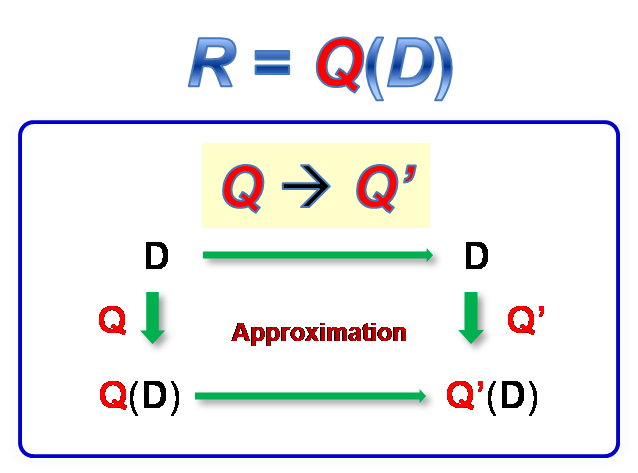
\includegraphics[scale=0.5]{./queryApprox.png}
  \end{center}
  \vspace{-3ex}
  \caption{Query approximation}\label{fig-tech-queryappro}
  \vspace{-2ex}
\end{figure}


\stitle{(1) Strong Simulation~\cite{tods-MaCFHW14}}. Given a pattern graph $Q$ and a data graph $G$,
{\em graph pattern matching} is to find all subgraphs of $G$ that match $Q$, and is being increasingly used in various applications, \eg software, biology, social networks and intelligence analysis.


Here {\em matching} is typically defined in terms of
{\em subgraph isomorphism} \cite{Galla06}:
a subgraph $G_s$ of $G$ {\em matches} $Q$ if
there exists a {\em bijective function} $f$
from the nodes of $Q$ to the nodes in $G_s$ such that (a)  for each
pattern node $u$ in $Q$, $u$ and $f(u)$
have the same label,
and (b) there exists an edge $(u, u')$ in $Q$ if and only
if there exists an edge $(f(u), f(u'))$ in $G_s$.


The goodness of subgraph isomorphism is that all matched subgraphs  are exactly the same as the pattern graph, \ie completely preserving the  topology structure between the pattern graph and data graph. However, subgraph isomorphism is \NP-complete, and may return exponential many matched subgraphs.
Further, subgraph isomorphism is too restrictive to find sensible matches in certain scenarios, as observed in~\cite{FanLMTWW10}. Even worse, online data in many cases only represents a partial world (\eg terrorist collaboration networks and homosexual networks often involve with a large amount of off-line data).
Exact computations on such online data, whose accompanying off-line data is extremely hard to gather, typically decreases the chance of identifying candidate answers.
These hinder the usability of graph pattern matching in emerging applications.


To lower the high complexity of subgraph isomorphism, substitutes for subgraph isomorphism \cite{FanLMTWW10,FanLMTW11}, which allow graph pattern matching to be conducted in cubic-time, have been proposed by extending graph simulation~\cite{infsimu95}. However, they fall short of capturing the topology of data graphs, i.e., graphs may have a structure drastically different from pattern graphs that they match, and the matches found are often too large to analyze.

To rectify these problems, strong simulation, an ``approximate'' substitute for subgraph isomorphism, is proposed for graph pattern matching~\cite{tods-MaCFHW14}, such that strong simulation (a) theoretically preserves the key topology of pattern graphs and finds a bounded number of matches, (b) retains the same complexity as earlier extensions of graph simulation~\cite{FanLMTWW10,FanLMTW11}, by providing a cubic-time algorithm for computing strong simulation, and (c) has the locality property that allows us to develop an effective distributed algorithm to conduct graph pattern matching on distributed graphs.

Strong simulation is experimentally verified that it is able to identify sensible matches that are not found by subgraph isomorphism, and it finds high
quality matches that retain graph topology. Indeed, 70\%-80\% of matches found by subgraph
isomorphism are retrieved by strong simulation. Further, strong simulation is over $100$ times faster than subgraph isomorphism, and has a bounded number of matches.



\stitle{(2) One-Pass Trajectory Compression~\cite{LinMZWH17}}.  Trajectory compression (\aka trajectory simplification) is to compress data points in a trajectory to a set of continuous line segments, and is commonly used  in practice.

Though lossless compression methods incur no information loss, their compression ratios are typically poor, and querying on the compressed data is time consuming due to the reconstruction of the original data \cite{Nibali:Trajic}. Hence, lossy techniques become the mainstream for trajectory compression,
which provide approximate solutions with good compression ratios and bounded errors in practice.


Piece-wise line simplification (\lsa) comes from computational geometry, whose target is to approximate a given finer piece-wise linear curve by another coarser piece-wise linear curve ({normally} a subset of the former), such that the maximum distance of the former from the later is bounded by a user specified constant. It is widely used due to its distinct advantages: (a) simple and easy to implement, (b) no need of extra knowledge and suitable for freely  moving  objects, and (c) bounded errors with good compression ratios.

\lsa algorithms fall into two categories: {\em optimal} and {\em approximate}.
Optimal methods\cite{Imai:Optimal} are to find the minimum number of points or segments to represent the original polygonal lines \wrt an error bound $\epsilon$. They have higher time and space complexities, and are not practical for large trajectory data.
Hence,  various approximate \lsa algorithms have been developed, from batch algorithms (\eg \cite{Douglas:Peucker}) to online algorithms (\eg~\cite{Liu:BQS}) and to one-pass algorithms (\eg~\cite{LinMZWH17}).


An \lsa algorithm is {\em one-pass} if it processes each point in a trajectory once and only once when compressing the trajectory.
Obviously, one-pass algorithms have low time and space complexities, and are more appropriate for online processing. The difficulty comes from the need to achieve effective compression ratios.
Existing trajectory simplification algorithms (\eg \cite{Douglas:Peucker}) and online algorithms  (\eg \cite{Liu:BQS}) essentially employ a global distance checking approach to assuring error bounds, although online algorithms restrict the checking within a window. That is to say, whenever a new directed line segment is formed, these algorithms always check its distances to all or a subset of data points, and, therefore, a data point is checked multiple times, depending on its order in the trajectory and the number of directed line segments formed. Hence, {\em an appropriate local distance checking approach is needed in the first place for designing one-pass trajectory simplification algorithms}.

 We develop a local distance checking method, referred to as  {\em fitting function}, such that a data point is checked only once during the entire process of trajectory simplification. Based on the fitting function, we develop one-pass error bounded trajectory simplification algorithms \operb and \operba that scan each data point in a trajectory once and only once, allowing interpolating new data points or not, respectively. By comparing our algorithms with \fbqsa (the fastest existing \lsa online algorithm \cite{Liu:BQS}) and \dpa (the best existing \lsa batch algorithm in terms of compression ratio \cite{Douglas:Peucker}), our one-pass algorithms  \operb and \operba are over four times faster than \fbqsa, and have  comparable compression ratios with \dpa.


\stitle{(3) Dense Temporal Subgraph Computation~\cite{MaHWLH17}}.  We study dense subgraphs in {\em a special type of temporal networks} such that their nodes and edges are kept fixed, but their edge weights constantly and regularly vary with timestamps~\cite{MaHWLH17}.  Essentially, a temporal network with $T$ timestamps can be viewed as $T$ snapshots of a static network such that the network nodes and edges are kept the same among these $T$ snapshots, while the edge weights vary with network snapthots. Road traffic networks typically fall into this category of temporal networks, and dense subgraphs are used for road traffic analyses that are of particular importance for large cities, such as Beijing, New York, London and Paris, that are facing with heavy traffic congestions, one of the great challenges in urban computing.

Dense subgraphs are a general concept, and their concrete semantics highly depend on the studied problems and applications. Though  dense subgraphs have been widely studied in static networks, how to properly define their semantics over temporal networks is still in the early stage, not to mention effective and efficient analytic algorithms.

We adopt the {\em form of dense temporal subgraphs} initially defined and studied in \cite{BogdanovMS11}, such that a temporal subgraph corresponds to a connected subgraph measured by the sum of all its edge weights in a time interval, \ie  a continuous sequence of timestamps. Intuitively, a dense subgraph that we consider  corresponds to a  collection of connected highly slow or jam roads (\ie  a jam area) in road networks, lasting for a continuous sequence of snapshots.


The problem of  finding dense subgraphs in temporal networks is non-trivial, and it is already \NP-complete even for a temporal network with a single snapshot and with $+1$ or $-1$ edge weights only, as observed in \cite{BogdanovMS11}. Even worse, it remains hard to approximate for temporal networks  with single snapshots~\cite{MaHWLH17}. Moreover, given a temporal network with $T$ timestamps, there are a total number of $T*(T+1)/2$ time intervals to consider, which further aggravates the difficulty. The state of the art solution \kw{MEDEN} \cite{BogdanovMS11} adopts a filter-and-verification ({\kw{FAV}) framework that {\em even if a large portion of time intervals are filtered, there often remain a large number of time intervals to verify}. Hence, this method is not big data friendly, and is not scalable when temporal networks have a large number of nodes/edges or a large number $T$ of timestamps.


We develop a data-driven approach, instead of filter-and-verification, to  identifying the most possible $k$ time intervals from $T \times (T + 1)/2$ time intervals, in which $T$ is the number of snapshots and k is a small constant, \eg 10. This is achieved by exploring the characteristics of time intervals involved with dense subgraphs based on the observation of {\em evolving convergence phenomenon} in traffic data, inspired by the convergent evolution in nature\footnote{\small \url{https://en.wikipedia.org/wiki/Convergent_evolution}}. That is, our method provides time intervals with probabilistic grantees, instead of exact ones like \kw{FAV}.   Using both real-life and synthetic data, we experimentally show that Our method \kw{FIDES} is over 1000 times faster than the state of the art solution  \kw{MEDEN}~\cite{BogdanovMS11}, while the quality of dense subgraphs found is comparable with  \kw{MEDEN} .


\section{Data Approximation}
\label{sec-data}






Big data has large volume, and, hence, the space complexity~\cite{CormenLRS01} of big data analytic tasks starts raising more concerns.
Given a class $Q$ of queries on data $D$, data approximation is to transform $D$ into smaller $D'$ such that $Q$ on $D'$ returns a sufficient or satisfiable approximate answer in a more efficient way. Further, it is typically common that query $Q$ needs to be (slightly) modified to $Q'$ to accommodate  the changes of $D$ to $D'$, as shown in Fig.~\ref{fig-tech-dataappro}. Similar to query approximation, data approximation needs to reach a balance between the query efficiency and answer quality.


The rationale behind data approximation has roots in the Pareto principle\footnote{\small \url{https://en.wikipedia.org/wiki/Pareto_principle}} that ``states that, for many events, roughly 80\% of the effects come from 20\% of the causes''. The critical thing for data approximation is to determine which part of data is relevant to tasks (belong to the 20\%).
 By this principle, for many big analytic tasks, one may only need to keep a small amount of the data to derive high quality answers.
For example, when we are to build a predictive model on the stock of razers for an online store based on the order history of customers, orders from men are good enough. While on the stock of lipsticks, those from women are good enough. That is to say,  it is not necessary to use the entire data for certain data analytic tasks.



However, it should be pointed out that there are data analytic tasks such that data approximation could not work well. For example, an online store needs to count the total number of goods in its catalog.  Essentially entire goods should be considered for this task, and if a (small) portion of goods are chosen, it is hard to have a satisfiable result.


We next explain data approximation computation in more detail using three different data analytic tasks.



\stitle{(1) Proxies for Shortest Paths and Distances~\cite{MaFLWCH16}}. Computing shortest paths and distances is one of the fundamental problems on graphs. We study the {\em node-to-node shortest path} ({\em distance}) problem on large graphs: given a weighted undirected graph $G(V, E)$ with non-negative edge weights, and two nodes of $G$, the source $s$ and the target $t$, find the shortest path (distance) from $s$ to $t$ in $G$. The Dijkstra's algorithm with Fibonacci heaps runs in $O(n\log n + m)$ due to Fredman \& Tarjan~\cite{CormenLRS01}, where $n$ and $m$ denote the numbers of nodes and edges in a graph, respectively, which remains asymptotically the fastest known solution on arbitrary undirected graphs with non-negative edge weights.
%The challenge of computing shortest paths on large graphs.
However, computing shortest  paths and distances remains a challenging problem, in terms of both time and space cost, on large-scale graphs. Hence, various optimizations have been developed to speed-up the computation.

To speed-up shortest  path and distance queries, we propose {\em proxies} that have the following properties:
%
(a) each proxy captures a set of nodes in a graph, referred to as \dra,
%
(b) a small number of proxies can represent a large number of nodes in a graph,
%
(c) shortest paths and distances involved within the set of nodes being represented by the same proxies can be answered efficiently, and,
%
(d) the proxies and the set of nodes being represented can be computed efficiently in {\em linear} time.



The framework for speeding-up shortest path and distance queries with proxies consists of modules preprocessing and query answering as follows.


\ni(a) {\em Preprocessing}: Given graph $G(V, E)$, it first computes all \dras and their maximal proxies in linear time, then it computes and stores all the shortest paths and distances between any node and its proxy. It finally computes the reduced subgraph $G'$ by removing all \dras, but keeping their proxies, from graph $G$.


\ni(b) {\em Query answering}. Given two nodes $s$ and $t$ in graph $G(V$, $E)$  and the pre-computed information, the query answering module essentially executes the following.

The shortest path $\path(s, t)$ = $\path(s, u_s)/$ $\path(u_s, u_t)/$ $\path(u_t, t)$, where $u_s$ and $u_t$ are the proxies of $s$ and $t$, respectively.
Here  $\path(s, u_s)$ and $\path(u_t, t)$ are pre-computed, and $\path(u_s, u_t)$ can be computed on the reduced subgraph $G'$ by invoking any existing
(\eg \ah~\cite{zhu2013shortest}).
%
The shortest distance $\dist(s, t)$ = $\dist(s, u_s)$ + $\dist(u_s, u_t)$ + $\dist(u_t, t)$ can be computed similarly.

We show experimentally show that about $1/3$  nodes of real-life social networks and road networks  are captured by by proxies, leaving $2/3$ in the reduced graphs.
Hence, we propose a light-weight data reduction technique for speeding-up (exact)  shortest path and distance queries on large weighted undirected graphs~\cite{MaFLWCH16}.




\begin{figure}[tb!]
  \vspace{-1ex}
  \begin{center}
  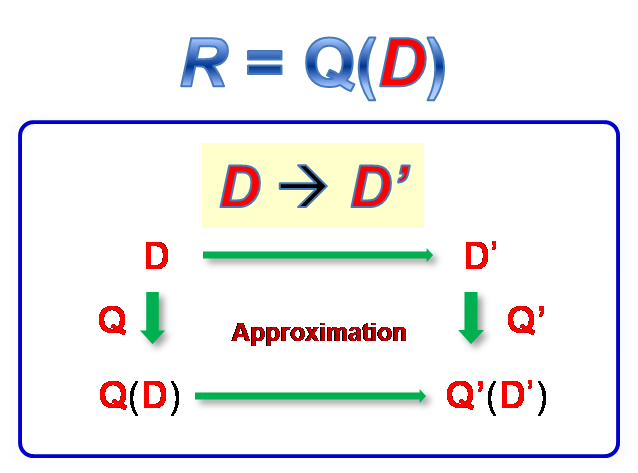
\includegraphics[scale=0.5]{./dataApprox.png}
  \end{center}
  \vspace{-3ex}
  \caption{Data approximation}\label{fig-tech-dataappro}
  \vspace{-2ex}
\end{figure}

\stitle{(2) Ensemble Enabled Link Prediction~\cite{DuanMAMH17}}. Link prediction is the task to predict the formation of future links in a dynamic and evolving network, and has been extensively studied due to its numerous applications, such as the recommendation of friends in a social network, images in a multimedia network, or
collaborators in a scientific network.


Link prediction methods are often applied to very large and sparse networks, which has a large {\em search space} $O(n^2)$,
where $n$ is the number of nodes. Hence, the scalability is a big challenge. In fact, an often overlooked fact is that most {\em exiting link prediction algorithms evaluate the link propensities only over a subset of possibilities rather than all propensities over the entire network},
\eg \cite{zhu2016}..
In order to understand why this is the case, consider a large network with $10^8$ nodes. Its number of {\em possibilities} for links
is of the order of $10^{16}$. Therefore, a 3GHz processor would
require at least $35$ days just to allocate one {\em machine cycle} to
every pair of nodes. This implies that in order to determine the
top-ranked link predictions over the {\em entire network}, the
running time will be much much larger than $35$ days.

It is noteworthy that most existing link prediction algorithms are not designed to search over the entire
$O(n^2)$ possibilities. A closer examination of the relevant
studies shows that even for networks of modest size, these
algorithms perform benchmark evaluations over a {\em
sample of the possibilities} for links.  In other
words, the {\em complete ranking problem for link prediction in
very large networks remains challenging at least from a
computational point of view}.


Latent factor models have been shown to be wildly successful in the domain of
collaborative filtering, but not link prediction in spite of the obvious
similarity between link prediction and collaborative filtering and
the obvious effectiveness of latent factor models. One of the reasons why latent factor models are rarely used for
link prediction is due to their complexity. In
collaborative filtering applications, the item dimension is of the
order of a few hundred thousand, whereas even the smallest  real-world networks contain more than a million nodes.
Even worse, we also experientially find that the quality of link prediction for latent factor models decreases with the increase of data sparsity,
and networks typically become sparser when their sizes grow larger.




\eat{%%%%%%%

The factorization of a matrix of
size $O(n^2)$ is not only computationally expensive, but also
memory-intensive.  As will be seen later in this article, one advantage
of  latent-factor models is that they are able to  transform the
adjacency matrix to a multidimensional space which can be searched
efficiently {\em by pruning} large portions of the $O(n^2)$ search
space in order to recommend the top-$k$ possibilities.

\begin{table}
\caption{The $O(n^2)$ problem in link prediction: Time required to
allocate a {\em single machine cycle} to every node-pair possibility
in networks of varying sizes and processors of various speeds.}
\label{time}
\vspace{0ex}
\centering
\begin{tabular}{cccc}
\hline \hline Network Sizes & 1 GHz &  3 GHz & 10 GHz \\
\hline \hline $10^6$ nodes & 1000 sec. & 333 sec. & 100 sec.\\
\hline $10^7$ nodes & 27.8 hrs &  9.3 hrs &  2.78 hrs\\
\hline $10^8$ nodes & $>100$ days &  $>35$ days & $> 10$ days\\
\hline $10^9$ nodes & $>10000$ days & $>3500$ days & $> 1000$ days\\
\hline \hline
\end{tabular}
\vspace{-2ex}
\end{table}
}%%%%%%%%%%%


We explore an {\em ensemble approach} to making latent factor models
practical for link prediction by decomposing the search space into a
 set of smaller matrices with three structural bagging methods with performance guarantees, which has obvious {\em
effectiveness} advantages. In this way, latent factor models only need to deal with networks with small sizes (and denser), and retain
their effectiveness and efficiency.  By incorporating with the characteristics of  link prediction, the bagging methods maintain high prediction
accuracy while reducing the network size via graph sampling techniques.
Further, the same bias-variance tradeoffs apply to the link-prediction problem, as the
standard classification problem. Therefore, the use of an ensemble
approach has obvious robustness advantages as well.


We experimentally show that our ensemble approach is over $50$ times faster and  over $20\%$ more accurate than {\sc bigclam} \cite{yang-wsdm2013} on using real-life social networks.


\eat{
\stitle{(1) Network Anomaly Detection~\cite{HuAMH16}}
We have adopted the idea in the process of dealing with large graphs in the study of anomaly detection in graph streams, when dealing with the matrix representation of a social graph, and  we have both theoretically and experimentally shown that simplifying the matrix by replacing a part of small entry values  with zero has few affects on the computation of eigenvectors~\cite{YuAMW13}.
}%%%%%%%%%%%%EAT







\section{Beyond Query and Data Approximation}
\label{sec-beyond}

  For big data analytics, there are no one-size-fits-all techniques, and it is often necessary to combine different techniques to obtain good solutions.


We have seen that data sampling helps to achieve a balance between efficiency and effectiveness for link prediction,
and other techniques such as incremental computation, data partitioning, data indexing and distributed computing can
also be unitized for big data analytics, and even for designing query and data approximation techniques for big data analytics.
For instance, it is easy to see that incremental algorithms (see~\cite{Reps96} for a survey) can be utilized to achieve query approximation.

It is also obvious that techniques beyond query and data approximation, such as theory and systems~\cite{FanGN13,Jordan15,ZahariaXWDADMRV16}, are must things for big data analytics.


\section{Conclusion}
\label{sec-conclusion}

In this article we have systematiclly introduced approximation computation techniques toward efficient and effective big data analytics.
Furthermore, although approximate computation does not put
theoretical bounds with respect to optimal solutions, it does expect a balance between efficiency and accuracy. Indeed, (1) our query approximation techniques~\cite{tods-MaCFHW14,LinMZWH17,MaHWLH17} show that efficiency can be obtained efficiency with high accuracy in practice, and (2) our data approximation techniques for shortest paths and distances and link prediction~\cite{MaFLWCH16,DuanMAMH17} show that efficiency and accuracy can be obtained for certain data analytic tasks. That is, the design policy approximate computation of is not to sacrifice accuracy for efficiency, but to achieve both efficiency and effectiveness in practice.





\stitle{Acknowledgement}. This work is supported in part by 973 program ({\small 2014CB340300}), NSFC ({\small U1636210 \& 61421003}). We would also thank our colleagues Charu Aggarwal, Gao Cong, Wenfei Fan, Chunming Hu, Xuelian Lin, Haixun Wang, Tianyu Wo and our students Yang Cao, Liang Duan, Kaiyu Feng, Renjun Hu, Han Zhang for their joined efforts.


\newpage
\balance
\bibliographystyle{abbrv}
\vspace{-1ex}
\begin{small}
\bibliography{paper}
\end{small}

\vspace{-4ex}
\begin{IEEEbiography}
%[{\includegraphics[width=1in,height=1.25in,clip,keepaspectratio]{bio/shuai-ma.eps}}]
{Shuai Ma} is a professor at the School of Computer Science and Engineering, Beihang University, China.
He obtained his PhD degrees from University of Edinburgh in 2010, and from
Peking University in 2004, respectively.
He was a postdoctoral research fellow in the database group, University of Edinburgh, a summer intern at Bell labs, Murray Hill, USA and a visiting researcher of MRSA.
He is a recipient of the best paper award for VLDB 2010 and the best challenge paper award for WISE 2013. His current research interests include database theory and systems, social data and graph analysis, and data intensive computing.
\end{IEEEbiography}
\vspace{-4ex}
\begin{IEEEbiography}
%[{\includegraphics[width=1in,height=1.25in,clip,keepaspectratio]{bio/jinpeng-huai.eps}}]
{Jinpeng Huai} is a professor at the School of Computer Science and Engineering, Beihang University, China. He received his Ph.D. degree in computer science from Beihang University, China, in 1993. Prof. Huai is an academician of Chinese Academy of Sciences and the vice honorary chairman of China Computer Federation (CCF). His research interests include big data computing, distributed systems, virtual computing, service-oriented computing, trustworthiness and security.
\end{IEEEbiography}

%}%%%%%%%%%%%%%%%%EAT%%%%%%%%%%%%%%%

\end{document}
